% Template for PLoS
% Version 3.5 March 2018
%
% % % % % % % % % % % % % % % % % % % % % %
%
% -- IMPORTANT NOTE
%
% This template contains comments intended
% to minimize problems and delays during our production
% process. Please follow the template instructions
% whenever possible.
%
% % % % % % % % % % % % % % % % % % % % % % %
%
% Once your paper is accepted for publication,
% PLEASE REMOVE ALL TRACKED CHANGES in this file
% and leave only the final text of your manuscript.
% PLOS recommends the use of latexdiff to track changes during review, as this will help to maintain a clean tex file.
% Visit https://www.ctan.org/pkg/latexdiff?lang=en for info or contact us at latex@plos.org.
%
%
% There are no restrictions on package use within the LaTeX files except that
% no packages listed in the template may be deleted.
%
% Please do not include colors or graphics in the text.
%
% The manuscript LaTeX source should be contained within a single file (do not use \input, \externaldocument, or similar commands).
%
% % % % % % % % % % % % % % % % % % % % % % %
%
% -- FIGURES AND TABLES
%
% Please include tables/figure captions directly after the paragraph where they are first cited in the text.
%
% DO NOT INCLUDE GRAPHICS IN YOUR MANUSCRIPT
% - Figures should be uploaded separately from your manuscript file.
% - Figures generated using LaTeX should be extracted and removed from the PDF before submission.
% - Figures containing multiple panels/subfigures must be combined into one image file before submission.
% For figure citations, please use "Fig" instead of "Figure".
% See http://journals.plos.org/plosone/s/figures for PLOS figure guidelines.
%
% Tables should be cell-based and may not contain:
% - spacing/line breaks within cells to alter layout or alignment
% - do not nest tabular environments (no tabular environments within tabular environments)
% - no graphics or colored text (cell background color/shading OK)
% See http://journals.plos.org/plosone/s/tables for table guidelines.
%
% For tables that exceed the width of the text column, use the adjustwidth environment as illustrated in the example table in text below.
%
% % % % % % % % % % % % % % % % % % % % % % % %
%
% -- EQUATIONS, MATH SYMBOLS, SUBSCRIPTS, AND SUPERSCRIPTS
%
% IMPORTANT
% Below are a few tips to help format your equations and other special characters according to our specifications. For more tips to help reduce the possibility of formatting errors during conversion, please see our LaTeX guidelines at http://journals.plos.org/plosone/s/latex
%
% For inline equations, please be sure to include all portions of an equation in the math environment.
%
% Do not include text that is not math in the math environment.
%
% Please add line breaks to long display equations when possible in order to fit size of the column.
%
% For inline equations, please do not include punctuation (commas, etc) within the math environment unless this is part of the equation.
%
% When adding superscript or subscripts outside of brackets/braces, please group using {}.
%
% Do not use \cal for caligraphic font.  Instead, use \mathcal{}
%
% % % % % % % % % % % % % % % % % % % % % % % %
%
% Please contact latex@plos.org with any questions.
%
% % % % % % % % % % % % % % % % % % % % % % % %

\documentclass[10pt,letterpaper]{article}
\usepackage[top=0.85in,left=2.75in,footskip=0.75in]{geometry}

% amsmath and amssymb packages, useful for mathematical formulas and symbols
\usepackage{amsmath,amssymb}

% Use adjustwidth environment to exceed column width (see example table in text)
\usepackage{changepage}


% textcomp package and marvosym package for additional characters
\usepackage{textcomp,marvosym}

% cite package, to clean up citations in the main text. Do not remove.
% \usepackage{cite}

% Use nameref to cite supporting information files (see Supporting Information section for more info)
\usepackage{nameref,hyperref}

% line numbers
\usepackage[right]{lineno}

% ligatures disabled
\usepackage{microtype}
\DisableLigatures[f]{encoding = *, family = * }

% color can be used to apply background shading to table cells only
\usepackage[table]{xcolor}

% array package and thick rules for tables
\usepackage{array}

% create "+" rule type for thick vertical lines
\newcolumntype{+}{!{\vrule width 2pt}}

% create \thickcline for thick horizontal lines of variable length
\newlength\savedwidth
\newcommand\thickcline[1]{%
  \noalign{\global\savedwidth\arrayrulewidth\global\arrayrulewidth 2pt}%
  \cline{#1}%
  \noalign{\vskip\arrayrulewidth}%
  \noalign{\global\arrayrulewidth\savedwidth}%
}

% \thickhline command for thick horizontal lines that span the table
\newcommand\thickhline{\noalign{\global\savedwidth\arrayrulewidth\global\arrayrulewidth 2pt}%
\hline
\noalign{\global\arrayrulewidth\savedwidth}}


% Remove comment for double spacing
%\usepackage{setspace}
%\doublespacing

% Text layout
\raggedright
\setlength{\parindent}{0.5cm}
\textwidth 5.25in
\textheight 8.75in

% Bold the 'Figure #' in the caption and separate it from the title/caption with a period
% Captions will be left justified
\usepackage[aboveskip=1pt,labelfont=bf,labelsep=period,justification=raggedright,singlelinecheck=off]{caption}
\renewcommand{\figurename}{Fig}

% Use the PLoS provided BiBTeX style
% \bibliographystyle{plos2015}

% Remove brackets from numbering in List of References
\makeatletter
\renewcommand{\@biblabel}[1]{\quad#1.}
\makeatother



% Header and Footer with logo
\usepackage{lastpage,fancyhdr,graphicx}
\usepackage{epstopdf}
%\pagestyle{myheadings}
\pagestyle{fancy}
\fancyhf{}
%\setlength{\headheight}{27.023pt}
%\lhead{
\includegraphics[width=2.0in]{PLOS-submission.eps}}
\rfoot{\thepage/\pageref{LastPage}}
\renewcommand{\headrulewidth}{0pt}
\renewcommand{\footrule}{\hrule height 2pt \vspace{2mm}}
\fancyheadoffset[L]{2.25in}
\fancyfootoffset[L]{2.25in}
\lfoot{\today}

%% Include all macros below

\newcommand{\lorem}{{\bf LOREM}}
\newcommand{\ipsum}{{\bf IPSUM}}


% tightlist command for lists without linebreak
\providecommand{\tightlist}{%
  \setlength{\itemsep}{0pt}\setlength{\parskip}{0pt}}


% Pandoc citation processing
%From Pandoc 3.1.8
% definitions for citeproc citations
\NewDocumentCommand\citeproctext{}{}
\NewDocumentCommand\citeproc{mm}{%
  \begingroup\def\citeproctext{#2}\cite{#1}\endgroup}
\makeatletter
 % allow citations to break across lines
 \let\@cite@ofmt\@firstofone
 % avoid brackets around text for \cite:
 \def\@biblabel#1{}
 \def\@cite#1#2{{#1\if@tempswa , #2\fi}}
\makeatother
\newlength{\cslhangindent}
\setlength{\cslhangindent}{1.5em}
\newlength{\csllabelwidth}
\setlength{\csllabelwidth}{3em}
\newenvironment{CSLReferences}[2] % #1 hanging-indent, #2 entry-spacing
 {\begin{list}{}{%
  \setlength{\itemindent}{0pt}
  \setlength{\leftmargin}{0pt}
  \setlength{\parsep}{0pt}
  % turn on hanging indent if param 1 is 1
  \ifodd #1
   \setlength{\leftmargin}{\cslhangindent}
   \setlength{\itemindent}{-1\cslhangindent}
  \fi
  % set entry spacing
  \setlength{\itemsep}{#2\baselineskip}}}
 {\end{list}}
\usepackage{calc}
\newcommand{\CSLBlock}[1]{#1\hfill\break}
\newcommand{\CSLLeftMargin}[1]{\parbox[t]{\csllabelwidth}{#1}}
\newcommand{\CSLRightInline}[1]{\parbox[t]{\linewidth - \csllabelwidth}{#1}\break}
\newcommand{\CSLIndent}[1]{\hspace{\cslhangindent}#1}

\usepackage[numbers]{natbib}
\usepackage{hyperref}
\usepackage[utf8]{inputenc}
\usepackage{capt-of}
\usepackage{booktabs}
\usepackage{amssymb}
\usepackage{threeparttable}
\usepackage{float}
%\floatplacement{figure}{H}
%\floatplacement{table}{H}
\usepackage{lipsum,caption}
\usepackage{pdflscape}



\usepackage{forarray}
\usepackage{xstring}
\newcommand{\getIndex}[2]{
  \ForEach{,}{\IfEq{#1}{\thislevelitem}{\number\thislevelcount\ExitForEach}{}}{#2}
}

\setcounter{secnumdepth}{0}

\newcommand{\getAff}[1]{
  \getIndex{#1}{spph,sp,stat}
}

\begin{document}
\vspace*{0.2in}


% Title must be 250 characters or less.
\begin{flushleft}
{\Large
\textbf\newline{Is There a Competitive Advantage to Using Multivariate
Statistical or Machine Learning Methods Over the Bross Formula in the
hdPS Framework for Bias and Variance
Estimation?} % Please use "sentence case" for title and headings (capitalize only the first word in a title (or heading), the first word in a subtitle (or subheading), and any proper nouns).
}
\newline
% Insert author names, affiliations and corresponding author email (do not include titles, positions, or degrees).
\\
Mohammad Ehsanul
Karim\textsuperscript{\getAff{spph}, \getAff{sp}}\textsuperscript{*},
Yang Lei\textsuperscript{\getAff{stat}}\\
\bigskip
\textbf{\getAff{spph}}School of Population and Public Health, University
of British Columbia, 2206 East Mall, Vancouver, V6T 1Z3, BC, Canada\\
\textbf{\getAff{sp}}St.~Paul's Hospital, 588 - 1081 Burrard Street,
Vancouver, V6Z 1Y6, BC, Canada\\
\textbf{\getAff{stat}}Department of Statistics, University of British
Columbia, Room 3182 Earth Sciences Building, 2207 Main Mall, Vancouver,
V6T 1Z4, BC, Canada\\
\bigskip
* Corresponding author: ehsan.karim@ubc.ca\\
\end{flushleft}
% Please keep the abstract below 300 words
\section*{Abstract}
\textbf{Purpose}: We aim to evaluate various proxy selection methods
within the context of high-dimensional propensity score (hdPS) analysis.
This study aimed to systematically evaluate and compare the performance
of traditional statistical methods and machine learning approaches
within the hdPS framework, focusing on key metrics such as bias,
standard error (SE), and coverage, under various exposure and outcome
prevalence scenarios. \textbf{Methods:} We conducted a plasmode
simulation study using data from the National Health and Nutrition
Examination Survey (NHANES) cycles from 2013 to 2018. We compared
methods including the kitchen sink model, Bross-based hdPS, Hybrid hdPS,
LASSO, Elastic Net, Random Forest, XGBoost, and Genetic Algorithm (GA).
The performance of each inverse probability weighted method was assessed
based on bias, MSE, coverage probability, and SE estimation across three
epidemiological scenarios: frequent exposure and outcome, rare exposure
and frequent outcome, and frequent exposure and rare outcome.
\textbf{Results:} XGBoost consistently demonstrated strong performance
in terms of MSE and coverage, making it effective for scenarios
prioritizing precision. However, it exhibited higher bias, particularly
in rare exposure scenarios, suggesting it is less suited when minimizing
bias is critical. In contrast, GA showed significant limitations, with
consistently high bias and MSE, making it the least reliable method.
Bross-based hdPS, and Hybrid hdPS methods provided a balanced approach,
with low bias and moderate MSE, though coverage varied depending on the
scenario. Rare outcome scenarios generally resulted in lower MSE and
better precision, while rare exposure scenarios were associated with
higher bias and MSE. Notably, traditional statistical approaches such as
forward selection and backward elimination performed comparably to more
sophisticated machine learning methods in terms of bias and coverage,
suggesting that these simpler approaches may be viable alternatives due
to their computational efficiency. \textbf{Conclusion:} The results
highlight the importance of selecting hdPS methods based on the specific
characteristics of the data, such as exposure and outcome prevalence.
While advanced machine learning methods such as XGBoost can enhance
precision, simpler methods such as forward selection or backward
elimination may offer similar performance in terms of bias and coverage
with fewer computational demands. Tailoring the choice of method to the
epidemiological scenario is essential for optimizing the balance between
bias reduction and precision.

% Please keep the Author Summary between 150 and 200 words
% Use first person. PLOS ONE authors please skip this step.
% Author Summary not valid for PLOS ONE submissions.

\linenumbers

% Use "Eq" instead of "Equation" for equation citations.
\section{Background}\label{background}

\textbf{High-dimensional Propensity Score (hdPS) Algorithm}: Propensity
scores are a crucial tool in causal inference for addressing
confounding. A propensity score is the conditional probability of
receiving a particular treatment or exposure, given a set of observed
covariates. Traditional propensity score models rely on
``investigator-specified'' or manually selected covariates based on
domain knowledge, prior literature, or theoretical frameworks.

In epidemiology, proxy variables are commonly used as substitutes for
confounders that are difficult or impossible to measure directly, such
as socioeconomic status, lifestyle factors, or health behaviors {[}1{]}.
These variables are not directly identified as confounders but serve as
surrogates for unmeasured or poorly measured confounders. The hdPS is a
pharmacoepidemiological method designed to reduce confounding bias in
large healthcare databases {[}2{]}. HdPS automatically ranks a wide
array of proxy variables from healthcare records---such as diagnosis
codes, medications, and procedures---using the Bross formula {[}3,4{]}.
The Bross formula ranks these variables based on their marginal
associations with both exposure and outcome. These selected proxy
variables serve as surrogates for unmeasured or poorly measured
confounders, helping reduce bias in treatment effect estimates. The hdPS
algorithm further refines the selection by prioritizing variables based
on their prevalence and potential for confounding, defined by their
association with both exposure and outcome {[}2{]}.

\textcolor{red}{Importantly, hdPS has become a foundational method in modern epidemiologic research that uses healthcare databases, offering a scalable and reproducible approach to confounding control when traditional investigator-specified propensity score models are limited by unmeasured, mismeasured, or omitted variables. Unlike conventional PS methods that rely solely on expert knowledge and a fixed set of covariates, hdPS empirically identifies and prioritizes proxy variables from high-dimensional data, allowing it to adjust for latent confounding structures more effectively. This makes hdPS particularly valuable for improving causal inference in observational healthcare studies, including those evaluating drug safety, treatment effectiveness, and health system interventions}
{[}5,6{]}.

\textbf{Multivariate Machine Learning Extensions}: Although the Bross
formula performs well in certain contexts, it has limitations in
capturing complex interactions, nonlinearities, and higher-order
associations between variables, especially in high-dimensional settings
where it does not account for the multivariate structure of other
covariates {[}5,7{]}. To address these model-specification-related
limitations, multivariate machine learning methods such as LASSO,
Elastic Net, and Random Forests have been applied within the hdPS
framework. These methods are better suited for high-dimensional data,
where they can more effectively handle complex relationships and improve
the selection of proxy variables, thus enhancing the precision of
treatment effect estimates {[}7--9{]}.
\textcolor{red}{Several studies have proposed hybrid approaches that combine machine learning and hdPS to enhance variable selection and bias reduction while maintaining interpretability}
{[}6,7,9{]}. Simulation studies and empirical research have shown that
these machine learning-based methods, or hybrid approaches combining the
Bross formula with machine learning, can reduce confounding more
effectively and increase efficiency compared to the Bross formula alone
in certain settings {[}7--9{]}.
\textcolor{red}{These efforts reflect a growing interest in refining hdPS with modern statistical learning tools to optimize proxy confounder adjustment in realistic, data-rich settings.}

\textbf{Assessing the Simulation Performance}: Other than bias, previous
studies have primarily focused on Mean Squared Error (MSE) as a key
metric for evaluating the performance of hdPS and its machine learning
extensions {[}7,9--12{]}. However, in high-dimensional settings with
singly robust methods, such as hdPS and machine learning approaches such
as LASSO, MSE may not always be the most reliable measure. MSE combines
both bias and variance into a single metric, which makes interpretation
challenging when variance estimation is unstable---a common issue in
these methods. In contrast, coverage, which measures the proportion of
confidence intervals that capture the true treatment effect, provides a
more direct and meaningful assessment of a model's reliability. In
realistic observational studies, where model misspecification is often
inevitable, coverage---along with related metrics such as
bias-eliminated coverage and relative error in standard error (SE; which
compares model-based SE with empirical SE)---can reveal whether
confidence intervals or SEs are too narrow (underestimating uncertainty)
or too wide (overestimating uncertainty). This insight is crucial in
determining whether the model delivers valid estimates despite
misspecification. Even a model with poor MSE but good coverage may still
be valuable, as it produces realistic confidence intervals. By shifting
the focus to coverage, rather than relying solely on MSE, we can achieve
a more comprehensive understanding of method performance, especially in
cases where unstable variance estimation might distort conclusions drawn
from MSE alone.
\textcolor{red}{To extend prior research, our study systematically compares multiple machine learning and hybrid hdPS approaches using plasmode simulations grounded in real-world data structure. Importantly, we expand beyond commonly reported metrics such as bias and MSE by incorporating underutilized diagnostics—namely, empirical coverage and relative error in standard error—to provide a more nuanced understanding of estimator performance.}

\textbf{Aim}: This research aims to systematically evaluate and compare
various proxy selection methods within the hdPS framework for inverse
probability weighted estimators, using a diverse range of simulation
performance metrics, including bias, MSE, and coverage. The study
focuses on assessing how these alternative statistical and machine
leartning methods perform in selecting proxy variables for confounding
adjustment, compared to the traditional Bross formula.

\section{Methods}\label{methods}

\subsection*{Data and Simulation}\label{data-and-simulation}
\addcontentsline{toc}{subsection}{Data and Simulation}

\textbf{Motivating Example}: We revisited the association between
obesity and the risk of diabetes using data from three cycles of the
National Health and Nutrition Examination Survey (NHANES) covering the
years 2013-2014, 2015-2016, and 2017-2018 {[}5{]}. To identify relevant
investigator-specified covariates, we constructed a causal diagram based
on literature {[}13--16{]} and established causal inference principles
{[}17{]}. The covariates included in our analysis were carefully
selected and categorized into demographic, behavioral, health history,
access-related, and laboratory variables. While most of these variables
were binary or categorical, the Laboratory variables were continuous.
The secondary, de-identified data used in this study were accessed from
the NHANES database on 1/5/2024-31/8/2024. The authors did not have
access to any information that could identify individual participants
during or after data collection. NHANES data are fully anonymized and
publicly available, ensuring that individual privacy is protected.

\textbf{Plasmode simulation}: To rigorously assess the performance of
the methods under consideration, we employed a plasmode simulation
framework, which is particularly well-suited for reflecting real-world
data structures and complexities {[}18{]}. This approach was inspired by
the analytic dataset derived from NHANES and involved resampling from
the observed covariates and exposure information (i.e., obesity) without
altering them. By mirroring key aspects of an actual epidemiological
study, this simulation framework offers a substantial advantage over
traditional Monte Carlo simulations, which often rely on hypothetical
assumptions.

\textbf{Simulation scenarios under consideration}: Our plasmode
simulation was conducted over 500 iterations. For the base simulation
scenario, we set the prevalence of exposure (obesity) and the event rate
(diabetes) at 30\%, with a true odds ratio (OR) parameter of 1,
corresponding to a risk difference (RD) of 0. Each simulated dataset had
a sample size of 3,000 participants. The description of other scenarios
under consideration is provided in Table \ref{table:scenarios}.

\begin{table}[ht]
\centering
\caption{Overview of Plasmode Simulation Scenarios Reflecting Varying Exposure and Outcome Prevalences Based on National Health and Nutrition Examination Survey (NHANES) Data Cycles (2013-2018)}
\label{table:scenarios}
\begin{tabular}{p{3cm}cccc}
  \toprule
  \textbf{Plasmode Simulation Scenario} & \textbf{Exposure} & \textbf{Outcome} & \textbf{True} & \textbf{Sample}\\
  \textbf{} & \textbf{Prevalence} & \textbf{Prevalence} & \textbf{Odds Ratio} & \textbf{Size}\\
  \midrule
  (i) Frequent Exposure and Outcome (Base) & 30\% & 30\% & 1 & 3,000 \\
  (ii) Rare Exposure and Frequent Outcome & 5\% & 30\% & 1 & 3,000 \\
  (iii) Frequent Exposure and Rare Outcome & 30\% & 5\% & 1 & 3,000 \\
  \bottomrule
\end{tabular}
\end{table}

\textbf{True Data Generating Mechanism Used in Plasmode Simulation}: The
primary goal of this plasmode simulation study is to evaluate various
variable selection methods under realistic conditions. To achieve this,
we formulated the outcome data based on a specific model specification
that incorporates both exposure and covariates, including
investigator-specified and proxy variables. The model specification
consists of three key components (See Appendices \S A and B for further
details):

\begin{enumerate}
\def\labelenumi{\arabic{enumi}.}
\item
  \emph{Investigator-Specified Covariates (demographic, behaviour and
  health history / access variables)}: We retained the original
  investigator-specified covariates, which were either binary or
  categorical, reflecting how real-world studies typically operate.
  These covariates were not included in the pool of proxy variables or
  subjected to any variable selection or ranking processes. Instead,
  they were always included in the analysis as a separate set of
  variables based on prior knowledge and causal reasoning. This ensured
  that these known confounders were appropriately accounted for,
  independent of the proxy variable selection framework.
\item
  \emph{Investigator-Specified Covariates (Transformation of Laboratory
  Variables)}: In real-world studies, it is common for analysts to lack
  precise knowledge of the true model specification. To simulate this
  uncertainty, we transformed the continuous laboratory variables using
  complex functions such as logarithmic, exponential, square root,
  polynomial transformations, and interactions. This reflects the
  challenges analysts face in correctly specifying models when dealing
  with continuous data.
\item
  \emph{Inclusion of Proxy Variables}: Real-world studies often deal
  with unmeasured confounding, which researchers attempt to mitigate by
  adding proxy variables. However, when a large number of proxies are
  added, some may act as noise variables, contributing little or nothing
  to the analysis. To simulate this, we selected only those binary proxy
  covariates (referred to as recurrence covariates in hdPS terminology)
  that had a relative risk (RR) of less than 0.8 or greater than 1.2
  concerning the outcome. Proxy variables were defined based on their
  association with the outcome because unmeasured confounders must
  influence the outcome to induce confounding. By prioritizing variables
  with strong outcome associations, we aimed to ensure that the proxies
  reflect at least part of the confounding structure. While not
  explicitly enforced, many of the selected proxy variables are expected
  to have some degree of association with the exposure.
\end{enumerate}

Out of 142 proxy covariates, 94 met this criterion and were summed in
calculating a simple comorbidity burden measure {[}19{]}. This score
represents the individual's overall comorbidity burden, reflecting the
cumulative presence of conditions. The remaining 48 covariates were
excluded from this calculation and considered noise. This comorbidity
burden measure (one variable) was then incorporated into our model
specification for generating the outcome data.

\textbf{Performance Measures}: From this simulation, we derived several
performance metrics to evaluate the effectiveness of the methods under
consideration: (1) bias, (2) average model-based SE (the average of
estimated SEs obtained from a model over repeated samples), (3)
empirical SE (the standard deviation of estimated treatment effects
across repeated samples), (4) MSE, (5) coverage probability of 95\%
confidence intervals, (6) bias-corrected coverage, and (7) Zip plot
{[}20,21{]}.

\subsection*{Inverse probability weighted estimators under
consideration}\label{inverse-probability-weighted-estimators-under-consideration}
\addcontentsline{toc}{subsection}{Inverse probability weighted
estimators under consideration}

The comparison between the data generation process and the analysis
process reveals two key differences: (i) The data generation used
transformed laboratory variables, whereas the analysis was conducted
using only the original laboratory variables. (ii) The data generation
employed a simple sum of selected proxy variables (sum of 94 proxy
covariates), while the analysis included all proxy variables (142 binary
proxies), with 48 of these acting as noise variables. These differences
help us assess how the proxy variable selection methods handle model
misspecification and the presence of noise variables.

We estimated propensity scores using the following models separately.
Propensity scores were then used to construct weights for each
individual, defined as the inverse of the probability of their observed
exposure status. The primary causal estimand of interest in this study
is the average treatment effect (ATE), which represents the difference
in expected outcomes between treated and untreated individuals if all
had been exposed to either treatment condition.

\begin{enumerate}
\def\labelenumi{\arabic{enumi}.}
\item
  \textbf{Kitchen sink model}: This is a base model for comparison,
  where no variable selection approaches were used. All
  investigator-selected features and all proxy variables were used to
  model {[}7{]}.
\item
  \textbf{hdPS using Bross formula}: The Bross formula is a statistical
  method used to calculate the bias introduced by not adjusting for a
  covariate {[}4{]}. In hdPS analysis, this formula was originally
  applied to each proxy variable to measure and rank the potential bias
  if the covariate were not adjusted for. In our analysis, the 100
  proxies with the highest bias rankings are selected for further
  modeling {[}2,3{]}.
\item
  \textbf{Least Absolute Shrinkage and Selection Operator (LASSO)}:
  LASSO is a variable selection technique that limits the number of
  variables by adding a penalty term to the regression model.
  Cross-validation (CV) is used in LASSO to identify variables with
  non-zero coefficients in the best model by optimizing the penalty
  value {[}7--9{]}.
\item
  \textbf{Hybrid of hdPS and LASSO}: Instead of relying solely on LASSO
  for variable selection, a hybrid approach combines the Bross formula
  and LASSO. First, proxy variables are selected using the hdPS
  algorithm (e.g., the top 100), and then LASSO is applied to further
  refine the selection {[}7,9{]}.
\item
  \textbf{Elastic Net}: Elastic Net is an extension of LASSO that
  includes an additional penalty term to handle multicollinearity by
  grouping correlated features and selecting the most representative
  ones {[}7{]}.
\item
  \textbf{Random Forest}: The Random Forest algorithm is an ensemble
  learning method that constructs multiple decision trees to perform
  classification {[}22{]}. It calculates the importance of each proxy
  variable based on the decrease in impurity or Gini importance,
  providing a ranking of the proxies. The top 100 variables from this
  ranking are manually selected for further modeling {[}8{]}.
\item
  \textbf{XGBoost}: XGBoost is a gradient boosting algorithm used to
  optimize machine learning models {[}23{]}. It builds decision trees
  that make splits based on maximum impurity reduction, and it assigns
  an importance score to each proxy variable by calculating the mean
  decrease in impurity {[}24{]}.
\item
  \textbf{Stepwise}: Stepwise selection is a progressive feature
  selection method that can proceed in two directions---forward or
  backward---based on the maximum adjusted R-squared. We have
  implemented two versions: (a) Forward selection (FS) starts with an
  initial model (e.g., including all investigator-selected features) and
  adds proxies to the model one at a time. (b) Backward elimination (BE)
  starts with a full model (e.g., all investigator-selected features and
  all proxy variables) and removes features one at a time based on their
  contribution to the model.
\item
  \textbf{Genetic algorithm}: Genetic algorithm is an evolutionary
  algorithm inspired by the theory of natural selection {[}25{]}. It
  operates by evolving offspring from a population of the fittest
  individuals over several generations, evaluating and selecting the
  best combination of features or variables that maximize prediction
  accuracy.
\end{enumerate}

\section{Results}\label{results}

The results for each method under the different scenarios are summarized
below. See Figures \ref{fig:bias-comparison} and
\ref{fig:Coverage-comparison} for an overview of the performance in
terms of bias and coverage, respectively. All simulation results can be
reviewed interactively through a Shiny web application available at
https://ehsanx.shinyapps.io/hdPS-Alternatives/, providing a convenient
platform for exploring the performance of each method across various
scenarios.

\begin{figure}

{\centering 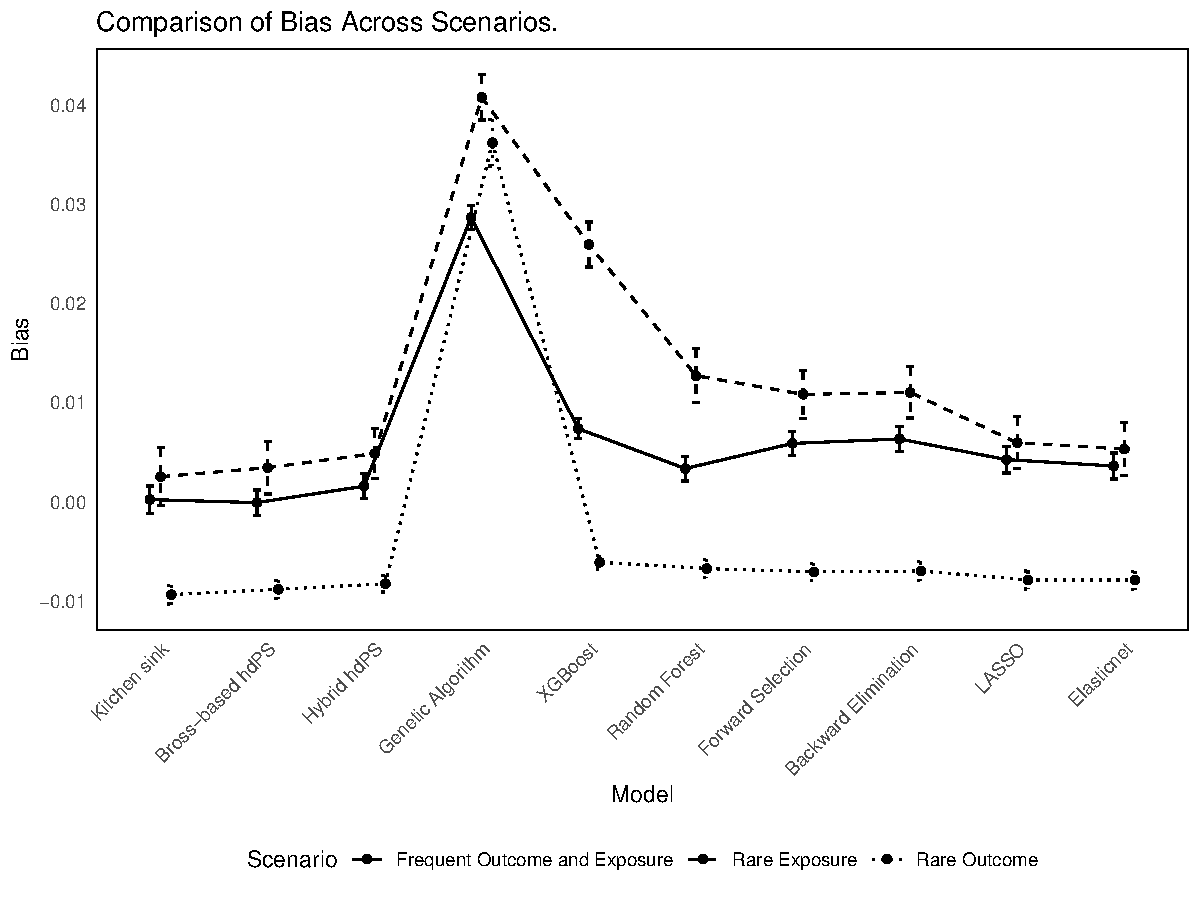
\includegraphics[width=1\linewidth]{figures/metric_comparison_BiasBW} 

}

\caption{Comparison of Bias Across Different Methods in hdPS Analysis\label{fig:bias-comparison}}\label{fig:unnamed-chunk-1}
\end{figure}

\begin{figure}

{\centering 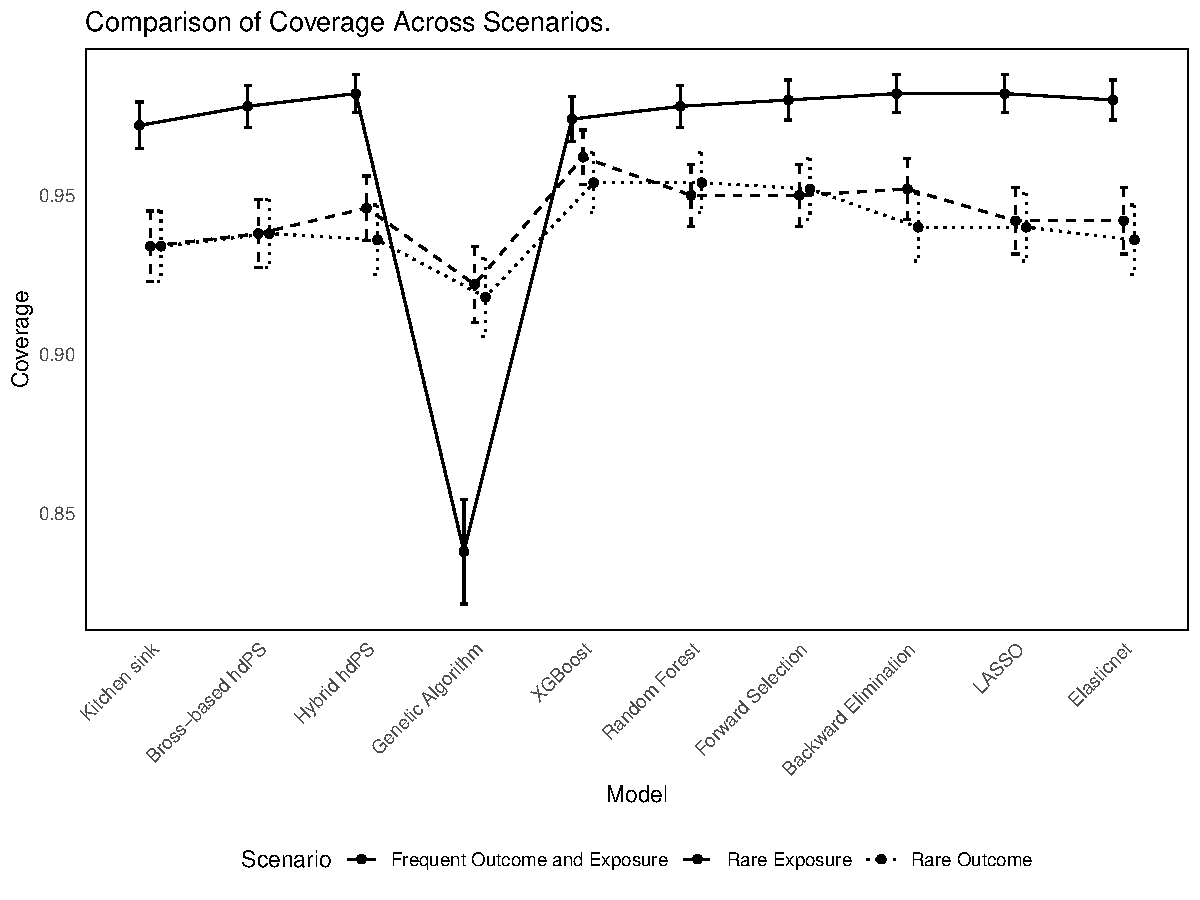
\includegraphics[width=1\linewidth]{figures/metric_comparison_CoverageBW} 

}

\caption{Comparison of Coverage Probability Across Different Methods in hdPS Analysis\label{fig:Coverage-comparison}}\label{fig:unnamed-chunk-2}
\end{figure}

\begin{enumerate}
\def\labelenumi{(\roman{enumi})}
\tightlist
\item
  \textbf{Frequent Exposure and Outcome (base) scenario}:
\end{enumerate}

\begin{enumerate}
\def\labelenumi{\arabic{enumi}.}
\item
  \emph{Bias}: Bross-based hdPS exhibited the smallest bias (-0.0001),
  and the kitchen sink model (0.0002) was the second. Genetic algorithm
  shows the highest bias (0.0287), indicating a substantial deviation
  from the true effect. Among the other methods, Hybrid hdPS (0.0016),
  and Elastic Net (0.0036) demonstrated low bias. XGBoost (0.0074) had
  slightly higher bias than Random Forest (0.0034).
\item
  \emph{Coverage}: The coverage for most methods was high, with Hybrid
  hdPS, Forward Selection, Backward Elimination, LASSO, and Elastic Net
  achieving values around 98\%, indicating well-calibrated confidence
  intervals. However, Genetic algorithm had noticeably lower coverage
  (83.8\%), indicating that its confidence intervals might be too narrow
  or biased, potentially missing the true effect. After applying bias
  elimination (as there were substantial bias associated with this
  method), Genetic algorithm's coverage improved to 96\%.
\item
  \emph{MSE}: XGBoost achieved the lowest MSE (0.0006). Genetic
  algorithm maintained the highest MSE (0.0016), reflecting its higher
  bias and variability. The kitchen sink model (0.0009), Bross-based
  hdPS (0.0008), Hybrid hdPS (0.0008), and Elastic Net (0.0009) all had
  relatively similar and moderate MSE values.
\item
  \emph{SE}: XGBoost exhibited the lowest Empirical SE (0.0229),
  indicating high precision in its estimates. The kitchen sink model had
  the highest Empirical SE (0.0305), suggesting greater variability.
  Other methods, including Genetic algorithm (0.0274), Hybrid hdPS
  (0.0278), and Bross-based hdPS (0.0287), showed moderate variability.
  LASSO (0.0299) and Elastic Net (0.0294) had slightly higher
  variability. The Model-based SE followed a similar pattern, with
  XGBoost (0.0268) showing the lowest variability and the kitchen sink
  model (0.0333) the highest, indicating less precision in its
  estimates. When comparing relative error in SE estimation, XGBoost
  performed the worst. See Appendix \S C for further details.
\end{enumerate}

\textbf{(ii) Rare Exposure and Frequent Outcome}:

\begin{enumerate}
\def\labelenumi{\arabic{enumi}.}
\item
  \emph{Bias}: The kitchen sink model showed a relatively low bias
  (0.0025), while Genetic algorithm continued to exhibit the highest
  bias (0.0408), indicating a significant deviation from the true
  effect. XGBoost had a bias of 0.0259, which, while still higher than
  other methods, but was lower than Genetic algorithm. Other methods,
  such as Bross-based hdPS (0.0035), Hybrid hdPS (0.0049), and Elastic
  Net (0.0053), demonstrated moderate bias. Random Forest (0.0127) and
  Forward Selection (0.0108) had slightly higher bias but remained
  within an acceptable range.
\item
  \emph{Coverage}: Coverage levels remained high for most methods, with
  XGBoost achieving the highest coverage at 96.2\%, indicating
  well-calibrated confidence intervals despite its higher bias. The
  Genetic algorithm method had lower coverage (92.2\%), suggesting that
  its confidence intervals might be narrower, potentially missing the
  true effect. Other methods such as RF, Forward Selection, Backward
  Elimination, and Hybrid hdPS maintained coverage values around
  94-95\%, suggesting adequate interval calibration. Bias-eliminated
  coverage for Genetic algorithm improved to 94.2\%, but it was still
  slightly lower than other methods (e.g., forward selection).
\item
  \emph{MSE}: Forward selection demonstrated the lowest MSE (0.0030),
  and then Hybrid hdPS and XGBoost. The Genetic algorithm method had a
  higher MSE (0.0043), reflecting its substantial bias and variability.
  The kitchen sink model also had an MSE of 0.0043, similar to Genetic
  algorithm, while other methods such as Bross-based hdPS (0.0035), RF
  (0.0039), and Elastic Net (0.0036) exhibited moderate MSE values,
  indicating reasonable accuracy.
\item
  \emph{SE}: The lowest Empirical SE was observed with XGBoost (0.0507)
  and Genetic algorithm (0.0510), reflecting high precision despite
  their higher bias. The kitchen sink model had the highest Empirical SE
  (0.0656), indicating greater variability. Hybrid hdPS (0.0564),
  Bross-based hdPS (0.0595), and RF (0.0609) showed moderate
  variability. Forward Selection (0.0537) and Backward Elimination
  (0.0576) had lower variability compared to the kitchen sink model. In
  terms of Model-based SE, XGBoost (0.0531) and Genetic algorithm
  (0.0533) continued to show low variability, while the kitchen sink
  model had the highest Model-based SE (0.0623), indicating less
  precision in its estimates. When comparing relative error in SE
  estimation, XGBoost and kitchen sink model performed the worst (in
  other direction).
\end{enumerate}

\textbf{(iii) Frequent Exposure and Rare Outcome}:

\begin{enumerate}
\def\labelenumi{\arabic{enumi}.}
\item
  \emph{Bias}: In this scenario, the kitchen sink model exhibited a
  moderate negative bias (-0.0093), similar to the Bross-based hdPS
  method (-0.0088). Genetic algorithm showed a significantly higher bias
  (0.0362), indicating a substantial deviation from the true effect.
  Among other methods, XGBoost demonstrated the lowest bias (-0.0061),
  while methods such as Hybrid hdPS (-0.0082), Forward Selection
  (-0.0070), and Backward Elimination (-0.0070) had slightly higher but
  still moderate biases. Elastic Net and LASSO both had biases of
  -0.0079, reflecting slightly larger deviations compared to XGBoost but
  still within acceptable limits.
\item
  \emph{Coverage}: Most methods achieved good coverage, with XGBoost,
  RF, and Forward Selection each achieving a coverage rate of 95.4\%,
  indicating well-calibrated confidence intervals. The Genetic algorithm
  method, however, had slightly lower coverage (91.8\%), indicating that
  its confidence intervals might be narrower, potentially excluding the
  true effect. Bross-based hdPS and the kitchen sink model had slightly
  lower coverage values of 93.8\% and 93.4\%, respectively. After
  accounting for bias, the bias-eliminated coverage for most methods,
  except Genetic algorithm, remained high, with values ranging from
  98.4\% to 99.0\%, indicating that most methods effectively adjusted
  for bias in their coverage estimates. Genetic algorithm's
  bias-eliminated coverage was lower at 93.4\%, reflecting its higher
  inherent bias.
\item
  \emph{MSE}: XGBoost exhibited the lowest MSE (0.0003). Genetic
  algorithm had the highest MSE (0.0040), reflecting its substantial
  bias and variability. The kitchen sink model (0.0005), Bross-based
  hdPS (0.0005), and other methods such as Hybrid hdPS (0.0004) and
  Elastic Net (0.0005) all had relatively similar MSE values, indicating
  moderate accuracy.
\item
  \emph{SE}: The lowest Empirical SE was observed with XGBoost (0.0152),
  reflecting high precision in its estimates. The Genetic algorithm
  method exhibited the highest Empirical SE (0.0523), indicating greater
  variability and less precision. Methods such as Hybrid hdPS (0.0184),
  Forward Selection (0.0187), and Elastic Net (0.0203) showed moderate
  variability, while Bross-based hdPS (0.0206) and the kitchen sink
  model (0.0212) had slightly higher variability. In terms of
  Model-based SE, XGBoost (0.0179) again showed the lowest variability,
  consistent with its low Empirical SE, indicating that it provided the
  most stable estimates. The kitchen sink model had a slightly higher
  Model-based SE (0.0219), indicating less precision in its estimates.
  When comparing relative error in SE estimation, XGBoost performed the
  worst.
\end{enumerate}

\section{Real-world analysis}\label{real-world-analysis}

\textbf{Summary results}: The dataset comprises 7,585 individuals. Among
these, the prevalence of the exposure is 48.8\%, while the prevalence of
the outcome is 23.7\%.

See Figure \ref{fig:comparison-plot-updated} for the results from
analyzing the NHANES (2013-2018) dataset. The methods are arranged
according to the number of selected proxy variables. Among all variable
selection algorithms, Random Forest and XGBoost demonstrate the highest
ORs, with values of 1.59 and 1.56, respectively. The ORs for the
remaining methods cluster around 1.52. Additionally, with the exception
of RF and the Bross formula hdPS, a general pattern emerges where
methods selecting a larger number of proxy variables yield lower ORs.
For RD, RF and XGBoost also exhibit the highest value 0.08, while the
remaining methods converge around 0.077. The trend observed in the OR
results appears to persist in the RD analysis.

\begin{figure}

{\centering 
\includegraphics{plos_files/figure-latex/unnamed-chunk-3-1} 

}

\caption{Figure presenting a comparison of Risk Differences (RD) and Odds Ratios (OR) with 95\% confidence intervals for different methods used to evaluate the association between obesity and diabetes risk. The analysis is based on data from the National Health and Nutrition Examination Survey (NHANES) for the years 2013-2018. Methods are arranged by the number of variables used in the models.\label{fig:comparison-plot-updated}}\label{fig:unnamed-chunk-3}
\end{figure}

Table \ref{tab:method-comparison-updated} presents a pairwise comparison
of the number of proxy features shared between different variable
selection methods used in the analysis. Each cell in the table indicates
the count of common proxy variables selected by the method in the
corresponding row and column. The diagonal cells, where the row and
column methods are the same, represent the total number of proxy
variables selected exclusively by each method. The first column displays
the number of proxy variables shared between each method and the kitchen
sink (KS) model. Given that the KS model includes all proxy variables,
the values in the first column are identical to those in the diagonal
cells for each row, which also presents the total number of proxy
variables selected by the method in the corresponding row.

\begin{landscape} 

\begin{table}[htbp]
\centering
\caption{Comparison of variable overlap of selected proxies across different methods used to evaluate the association between obesity and diabetes from the National Health and Nutrition Examination Survey (NHANES) for the years 2013-2018.}
\label{tab:method-comparison-updated}
\begin{tabular}{lcccccccccc}
\toprule
 & \textbf{KS} & \textbf{Bross} & \textbf{Hybrid} & \textbf{LASSO} & \textbf{EN} & \textbf{RF} & \textbf{XGB} & \textbf{FS} & \textbf{BE} & \textbf{GA} \\
\midrule
\textbf{Kitchen sink (KS)} & 142 & & & & & & & & & \\
\textbf{Bross formula} & 100 & 100 & & & & & & & & \\
\textbf{Hybrid (Bross and LASSO)} & 49 & 49 & 49 & & & & & & & \\
\textbf{LASSO} & 60 & 47 & 47 & 60 & & & & & & \\
\textbf{Elastic Net (EN)} & 69 & 54 & 48 & 60 & 69 & & & & & \\
\textbf{Random Forest (RF)} & 100 & 71 & 38 & 46 & 52 & 100 & & & & \\  
\textbf{XGBoost (XGB)} & 48 & 38 & 24 & 28 & 30 & 37 & 48 & & & \\
\textbf{Forward selection (FS)} & 59 & 45 & 41 & 51 & 54 & 45 & 25 & 59 & & \\
\textbf{Backward elimination (BE)} & 59 & 45 & 41 & 51 & 54 & 45 & 25 & 59 & 59 & \\
\textbf{Genetic algorithm (GA)} & 64 & 44 & 28 & 36 & 40 & 49 & 25 & 35 & 35 & 64 \\
\bottomrule
\end{tabular}
\end{table}

\end{landscape}

Table \ref{tab:proxy-common-pct-bross} presents a comparison of the
count and percentage of common proxy variables selected by different
methods in comparison with the Bross formula hdPS. The first column
shows the total number of proxy variables selected by each method, while
the second column lists the number of common features selected by both
the respective method and the Bross formula. The third column reports
the percentage of common features out of the total number of features
selected by each method.

We observe that, aside from the Bross formula hdPS and Random Forest
models, where the number of proxies was manually set to 100, and the
kitchen sink (KS) model, which includes all proxies by design, the
number of proxy variables selected by other models ranges between 49 and
69. As expected, the hybrid method combining Bross and LASSO hdPS
selects exactly 49 proxy variables, all of which are selected by both
methods, resulting in a common feature rate of 1.00. For other models,
the common feature percentage is generally clustered around \(74\%\),
with XGBoost showing the highest common percentage at \(79\%\), while
the Genetic Algorithm (GA) displays the lowest common percentage at
\(69\%\).

\begin{table}[htbp]
\centering
\caption{Comparison of the count and percentage of proxy variables selected by each methods in common with that by the Bross formula-based high-dimensional propensity score to evaluate the association between obesity and diabetes from the National Health and Nutrition Examination Survey (NHANES) for the years 2013-2018.}
\label{tab:proxy-common-pct-bross}
\begin{tabular}{p{4cm}ccc}
\toprule
\textbf{Method} & \textbf{Total Count} & \textbf{Common Count} & \textbf{Rate in Common} \\ 
\midrule
\textbf{Kitchen sink} & 142 & - & - \\
\textbf{Bross formula} & 100 & - & - \\
\textbf{Hybrid (Bross and LASSO)} & 49 & 49 & 1.00 \\
\textbf{LASSO} & 60 & 47 & 0.78 \\
\textbf{Elastic Net} & 69 & 54 & 0.78 \\
\textbf{Random Forest} & 100 & 71 & 0.71 \\  
\textbf{XGBoost} & 48 & 38 & 0.79 \\
\textbf{Forward selection} & 59 & 45 & 0.76 \\
\textbf{Backward elimination} & 59 & 45 & 0.76 \\
\textbf{Genetic algorithm} & 64 & 44 & 0.69 \\
\bottomrule
\end{tabular}
\end{table}

\textbf{Computing time}:

Figure \ref{fig:computing-time} presents the computing time for each
method. All methods, aside from RF and GA, exhibit relatively fast
computing times. RF and GA are generally much slower.

\begin{figure}

{\centering 
\includegraphics{plos_files/figure-latex/unnamed-chunk-4-1} 

}

\caption{Computing time for the real-world analysis for each algorithm under consideration. The analysis is based on data from the National Health and Nutrition Examination Survey (NHANES) for the years 2013-2018.\label{fig:computing-time}}\label{fig:unnamed-chunk-4}
\end{figure}

\section{Discussion}\label{discussion}

\subsection{Summary of the simulation
findings}\label{summary-of-the-simulation-findings}

\textbf{Comparison of methods}:

Across the three scenarios, XGBoost consistently achieved the lowest MSE
and high coverage, making it one of the most reliable methods in terms
of precision. However, it consistently exhibited some degree of bias,
particularly when compared to methods such as the kitchen sink model,
Bross-based hdPS, and Hybrid hdPS, which often showed lower bias in
scenarios with frequent outcomes. In contrast, GA displayed the highest
bias and MSE, along with lower coverage and greater variability, making
it the least reliable method for accurate effect estimation. Methods
such as Bross-based hdPS, Hybrid hdPS, and Elastic Net performed
moderately well across all scenarios, balancing bias, coverage, and MSE.
However, these methods did not outperform XGBoost in terms of overall
precision, especially with respect to MSE, though they often resulted in
lower bias. The kitchen sink model performed comparably to Bross-based
hdPS in terms of bias and coverage but lagged in SE estimation and MSE.

\textbf{Comparison of scenarios}:

In scenarios with rare exposure, higher bias was observed, particularly
for methods such as GA and XGBoost, whereas frequent outcomes generally
led to lower bias across most methods. Overcoverage was more common in
the scenario with frequent exposure and outcome, with several methods
producing confidence intervals that were too wide, suggesting an
overestimation of uncertainty. The other scenarios exhibited more
balanced or slightly under-coverage. Scenarios with frequent exposure
also displayed higher relative error in SE estimation, making it more
difficult to precisely estimate effects. In contrast, rare exposure
scenarios were associated with higher MSE, reflecting the challenge of
estimating effects when the exposure is uncommon. Rare outcome scenarios
exhibited the lowest MSE across most methods (except GA), indicating
that these scenarios provided a better balance between bias and
precision for most methods.

\subsection{Contextualizing the
literature}\label{contextualizing-the-literature}

Previous studies have shown that LASSO performs well within the hdPS
framework, particularly in terms of bias reduction and MSE {[}7,9{]},
with similar results for Elastic Net {[}7{]}. Our findings largely
support these conclusions, as both methods demonstrated moderate bias
and MSE across the scenarios. However, their performance was
inconsistent in some cases, with higher bias observed in rare exposure
scenarios, as noted in previous studies {[}7,9{]}. MSE also increased in
rare exposure scenarios. The Hybrid hdPS method, combining Bross-based
hdPS and LASSO, showed promising results, especially in terms of MSE,
suggesting it may serve as a suitable alternative to traditional hdPS
methods. Random Forest also performed similarly in our study, yielding
relatively low bias, which is consistent with previous findings {[}7{]}.
However, none of the earlier works emphasized coverage or examined
methods such as GA, XGBoost, forward selection, or backward elimination,
which were evaluated here.

\subsection{Data analysis findings}\label{data-analysis-findings}

The real-world dataset, with frequent exposure (48.8\%) and a moderate
outcome rate (23.7\%), produced ORs of 1.59 and 1.56 for RF and XGBoost,
respectively, while other methods clustered around an OR of 1.52. A
general trend emerged, showing that methods selecting fewer proxy
variables yielded lower ORs, except for RF and the Bross formula hdPS.
In terms of risk difference (RD), estimates were relatively stable
across methods. Regarding variable overlap, most methods shared around
74\% of their proxy variables with the Bross formula hdPS, with XGBoost
showing the highest common rate (79\%) and GA the lowest (69\%).
Computing time analysis showed that, aside from RF and GA, most methods
had relatively fast computing times, with RF being significantly slower.

\subsection{Strengths}\label{strengths}

Previous studies on singly robust methods have mainly focused on hdPS
performance using MSE as the primary evaluation metric {[}7,9--12{]}.
Our study extends this body of work by incorporating a broader range of
performance metrics, allowing researchers to compare results in terms of
both bias and variance estimation. This comprehensive comparison of
statistical and machine learning methods across various scenarios has
not been conducted before. For instance, we found that while XGBoost
consistently demonstrated strong performance in terms of MSE and
coverage, it did not always have the lowest bias. Additionally, we
observed that traditional variable selection methods such as forward
selection and backward elimination performed similarly to more
sophisticated methods such as LASSO and Random Forest across scenarios,
both in terms of bias and coverage.

Our study also employed a complex plasmode simulation framework, closely
replicating real-world data conditions {[}18{]}. This framework not only
accounted for model misspecification, where the true relationships
between covariates and outcomes were unknown, but also introduced noise
variables, addressing the challenge of dealing with irrelevant
covariates in high-dimensional settings. By applying transformations to
continuous variables and adding proxy variables that contributed
minimally to the outcome, we rigorously evaluated how well each method
handled both model uncertainty and non-informative variables, further
strengthening the real-world relevance of our findings.

\subsection{Future Direction}\label{future-direction}

Double robust methods have demonstrated strong potential for achieving
optimal statistical performance in hdPS analyses {[}10,26,27{]}. In
addition, single robust methods, such as ensemble learners such as super
learners, have shown promise in improving bias, MSE, area under the
curve (AUC), and covariate balance in other contexts {[}11,28,29{]}.
Deep learning methods, particularly supervised architectures, offer
significant potential for improving propensity score estimation in
high-dimensional settings by capturing complex, non-linear relationships
and performing well in scenarios with rare exposures, while maintaining
comparable bias and superior variance estimation compared to traditional
methods {[}30{]}. Despite their theoretical advantages, the complexity
and computational demands of these methods, especially in
high-dimensional settings, have limited their adoption by practitioners.
On the other hand, the simpler singly robust machine learning methods
evaluated here have been applied in clinical research {[}31,32{]}.

Future research should explore the application of double robust methods
and super learners in hdPS analyses, particularly for handling rare
outcomes and exposures, where the performance of traditional methods may
be suboptimal. Additionally, investigating the impact of different
hyperparameters on machine learning methods such as XGBoost could
optimize their performance in hdPS analysis. Finally, future simulation
studies should focus on evaluating coverage and other metrics in
epidemiological scenarios such as time-varying exposures, which would
provide valuable insights into the generalizability of our findings
{[}33{]}.

\subsection{Conclusion}\label{conclusion}

In conclusion, this analysis highlights the importance of carefully
selecting appropriate methods for hdPS analysis based on the specific
characteristics of the data, particularly the prevalence of exposure and
outcome. These findings also emphasize the need to tailor method
selection to the specific epidemiological scenario, ensuring that the
chosen method aligns with the study's goals, whether minimizing bias or
maximizing precision.

XGBoost consistently demonstrated strong performance in terms of MSE and
coverage, making it an effective choice when precision is prioritized.
However, it did not achieve the lowest bias, particularly in rare
exposure scenarios, indicating that it may be less suited when
minimizing bias is the primary objective. In contrast, the Genetic
Algorithm (GA) exhibited significant limitations, with consistently high
bias and MSE, making it less reliable for effect estimation.

The kitchen sink, Bross-based hdPS, and Hybrid hdPS methods provided a
more balanced approach, offering low bias and moderate MSE, though
coverage varied depending on the scenario. The analysis also revealed
that rare outcomes were associated with lower MSE and better precision,
while rare exposures presented challenges, yielding higher bias and MSE.
Interestingly, traditional statistical approaches such as forward
selection and backward elimination performed comparably to more
sophisticated machine learning methods across many scenarios. This
suggests that simpler approaches can still be viable, particularly in
terms of bias and coverage, and might be preferred due to their
computational efficiency.

\section*{List of abbreviations}\label{list-of-abbreviations}
\addcontentsline{toc}{section}{List of abbreviations}

\begin{itemize}
\tightlist
\item
  hdPS: High-dimensional Propensity Score
\item
  NHANES: National Health and Nutrition Examination Survey
\item
  OR: Odds Ratio
\item
  RD: Risk Difference
\item
  SE: Standard Error
\item
  MSE: Mean Squared Error
\item
  KS: Kitchen Sink
\item
  LASSO: Least Absolute Shrinkage and Selection Operator
\item
  EN: Elastic Net; a regularized regression method that combines LASSO
  and Ridge regression
\item
  RF: Random Forest
\item
  XGBoost: Extreme Gradient Boosting
\item
  FS: Forward Selection
\item
  BE: Backward Elimination
\item
  GA: Genetic Algorithm
\item
  CV: Cross-Validation
\item
  RR: Relative Risk
\end{itemize}

\section*{Declarations}\label{declarations}
\addcontentsline{toc}{section}{Declarations}

\subsection*{Ethics approval and consent to
participate}\label{ethics-approval-and-consent-to-participate}
\addcontentsline{toc}{subsection}{Ethics approval and consent to
participate}

The analysis conducted on secondary and de-identified data is exempt
from research ethics approval requirements. Ethics for this study was
covered by item 7.10.3 in University of British Columbia's Policy \#89:
Research and Other Studies Involving Human Subjects 19 and Article 2.2
in of the Tri-Council Policy Statement: Ethical Conduct for Research
Involving Humans (TCPS2).

\subsection*{Consent for publication}\label{consent-for-publication}
\addcontentsline{toc}{subsection}{Consent for publication}

The National Health and Nutrition Examination Survey (NHANES), conducted
by the U.S. Centers for Disease Control and Prevention (CDC), involves
collecting data through direct physical examinations, laboratory
testing, and interviews. The CDC already obtains consent from
participants when collecting this data. When researchers use NHANES data
for their studies, they are typically using de-identified, publicly
available data. This means that the information cannot be linked back to
individual participants, and therefore, additional consent from
participants is not required for researchers to use this data.

\subsection*{Availability of data and
materials}\label{availability-of-data-and-materials}
\addcontentsline{toc}{subsection}{Availability of data and materials}

NHANES data is publicly accessible and can be retrieved from the NHANES
website. The datasets generated and/or analyzed during the current study
are available in the NHANES repository:
https://www.cdc.gov/nchs/nhanes/index.htm. Additionally, all simulation
results can be interactively reviewed through a Shiny web application at
https://ehsanx.shinyapps.io/hdPS-Alternatives/.

\subsection*{Clinical trial number}\label{clinical-trial-number}
\addcontentsline{toc}{subsection}{Clinical trial number}

Not applicable.

\subsection*{Competing interests}\label{competing-interests}
\addcontentsline{toc}{subsection}{Competing interests}

MEK is currently supported by grants from Canadian Institutes of Health
Research and MS Canada. MEK has previously received consulting fees from
Biogen Inc.~for consulting unrelated to this current work. MEK was also
previously supported by the Michael Smith Foundation for Health Research
Scholar award.

\subsection*{Funding}\label{funding}
\addcontentsline{toc}{subsection}{Funding}

This work was supported by MEK's Natural Sciences and Engineering
Research Council of Canada (NSERC) Discovery Grant (PG\#: 20R01603) and
Discovery Launch Supplement (PG\#: 20R12709).

\subsection*{Authors' contributions}\label{authors-contributions}
\addcontentsline{toc}{subsection}{Authors' contributions}

MEK: Conceptualization, Writing -- Original Draft, Review \& Editing YL:
Formal Analysis, Review \& Editing

\subsection*{Acknowledgements}\label{acknowledgements}
\addcontentsline{toc}{subsection}{Acknowledgements}

Not applicable.

\section*{References}\label{references}
\addcontentsline{toc}{section}{References}

\phantomsection\label{refs}
\begin{CSLReferences}{0}{1}
\bibitem[\citeproctext]{ref-vanderweele2019principles}
\CSLLeftMargin{1. }%
\CSLRightInline{VanderWeele TJ. Principles of confounder selection.
European journal of epidemiology. 2019;34: 211--219. }

\bibitem[\citeproctext]{ref-schneeweiss2009high}
\CSLLeftMargin{2. }%
\CSLRightInline{Schneeweiss S, Rassen JA, Glynn RJ, Avorn J, Mogun H,
Brookhart MA. High-dimensional propensity score adjustment in studies of
treatment effects using health care claims data. Epidemiology
(Cambridge, Mass). 2009;20: 512. }

\bibitem[\citeproctext]{ref-wyss2018erratum}
\CSLLeftMargin{3. }%
\CSLRightInline{Wyss R, Fireman B, Rassen JA, Schneeweiss S. Erratum:
High-dimensional propensity score adjustment in studies of treatment
effects using health care claims data. Epidemiology. 2018;29: e63--e64.
}

\bibitem[\citeproctext]{ref-bross1966spurious}
\CSLLeftMargin{4. }%
\CSLRightInline{Bross ID. Spurious effects from an extraneous variable.
Journal of chronic diseases. 1966;19: 637--647. }

\bibitem[\citeproctext]{ref-karim2024high}
\CSLLeftMargin{5. }%
\CSLRightInline{Karim ME. High-dimensional propensity score and its
machine learning extensions in residual confounding control. The
American Statistician. 2024; 1--38. }

\bibitem[\citeproctext]{ref-wyss2022machine}
\CSLLeftMargin{6. }%
\CSLRightInline{Wyss R, Yanover C, El-Hay T, Bennett D, Platt RW, Zullo
AR, et al. Machine learning for improving high-dimensional proxy
confounder adjustment in healthcare database studies: An overview of the
current literature. Pharmacoepidemiology and Drug Safety. 2022;31:
932--943. }

\bibitem[\citeproctext]{ref-karim2018can}
\CSLLeftMargin{7. }%
\CSLRightInline{Karim ME, Pang M, Platt RW. Can we train machine
learning methods to outperform the high-dimensional propensity score
algorithm? Epidemiology. 2018;29: 191--198. }

\bibitem[\citeproctext]{ref-schneeweiss2017variable}
\CSLLeftMargin{8. }%
\CSLRightInline{Schneeweiss S, Eddings W, Glynn RJ, Patorno E, Rassen J,
Franklin JM. Variable selection for confounding adjustment in
high-dimensional covariate spaces when analyzing healthcare databases.
Epidemiology. 2017;28: 237--248. }

\bibitem[\citeproctext]{ref-franklin2015regularized}
\CSLLeftMargin{9. }%
\CSLRightInline{Franklin JM, Eddings W, Glynn RJ, Schneeweiss S.
Regularized regression versus the high-dimensional propensity score for
confounding adjustment in secondary database analyses. American journal
of epidemiology. 2015;182: 651--659. }

\bibitem[\citeproctext]{ref-pang2016effect}
\CSLLeftMargin{10. }%
\CSLRightInline{Pang M, Schuster T, Filion KB, Schnitzer ME, Eberg M,
Platt RW. Effect estimation in point-exposure studies with binary
outcomes and high-dimensional covariate data--a comparison of targeted
maximum likelihood estimation and inverse probability of treatment
weighting. The international journal of biostatistics. 2016;12. }

\bibitem[\citeproctext]{ref-wyss2018using}
\CSLLeftMargin{11. }%
\CSLRightInline{Wyss R, Schneeweiss S, Van Der Laan M, Lendle SD, Ju C,
Franklin JM. Using super learner prediction modeling to improve
high-dimensional propensity score estimation. Epidemiology. 2018;29:
96--106. }

\bibitem[\citeproctext]{ref-simon2023evaluating}
\CSLLeftMargin{12. }%
\CSLRightInline{Simon V, Vadel J. Evaluating the performance of
high-dimensional propensity scores compared with standard propensity
scores for comparing antihypertensive therapies in the CPRD GOLD
database. Cardiology and Therapy. 2023;12: 393--408. }

\bibitem[\citeproctext]{ref-saydah2014trends}
\CSLLeftMargin{13. }%
\CSLRightInline{Saydah S, Bullard KM, Cheng Y, Ali MK, Gregg EW, Geiss
L, et al. Trends in cardiovascular disease risk factors by obesity level
in adults in the united states, NHANES 1999-2010. Obesity. 2014;22:
1888--1895. }

\bibitem[\citeproctext]{ref-liu2013association}
\CSLLeftMargin{14. }%
\CSLRightInline{Liu J, Hay J, Faught BE, et al. The association of sleep
disorder, obesity status, and diabetes mellitus among US adults---the
NHANES 2009-2010 survey results. International journal of endocrinology.
2013;2013. }

\bibitem[\citeproctext]{ref-kabadi2012joint}
\CSLLeftMargin{15. }%
\CSLRightInline{Kabadi SM, Lee BK, Liu L. Joint effects of obesity and
vitamin d insufficiency on insulin resistance and type 2 diabetes:
Results from the NHANES 2001--2006. Diabetes care. 2012;35: 2048--2054.
}

\bibitem[\citeproctext]{ref-ostchega2012abdominal}
\CSLLeftMargin{16. }%
\CSLRightInline{Ostchega Y, Hughes JP, Terry A, Fakhouri TH, Miller I.
Abdominal obesity, body mass index, and hypertension in US adults:
NHANES 2007--2010. American journal of hypertension. 2012;25:
1271--1278. }

\bibitem[\citeproctext]{ref-greenland1999causal}
\CSLLeftMargin{17. }%
\CSLRightInline{Greenland S, Pearl J, Robins JM. Causal diagrams for
epidemiologic research. Epidemiology. 1999; 37--48. }

\bibitem[\citeproctext]{ref-franklin2014plasmode}
\CSLLeftMargin{18. }%
\CSLRightInline{Franklin JM, Schneeweiss S, Polinski JM, Rassen JA.
Plasmode simulation for the evaluation of pharmacoepidemiologic methods
in complex healthcare databases. Computational statistics and data
analysis. 2014;72: 219--226. }

\bibitem[\citeproctext]{ref-farley2006comparison}
\CSLLeftMargin{19. }%
\CSLRightInline{Farley JF, Harley CR, Devine JW. A comparison of
comorbidity measurements to predict healthcare expenditures. American
Journal of Managed Care. 2006;12: 110--118. }

\bibitem[\citeproctext]{ref-morris2019using}
\CSLLeftMargin{20. }%
\CSLRightInline{Morris TP, White IR, Crowther MJ. Using simulation
studies to evaluate statistical methods. Statistics in medicine.
2019;38: 2074--2102. }

\bibitem[\citeproctext]{ref-white2023check}
\CSLLeftMargin{21. }%
\CSLRightInline{White IR, Pham TM, Quartagno M, Morris TP. How to check
a simulation study. International Journal of Epidemiology. 2023;
dyad134. }

\bibitem[\citeproctext]{ref-breiman2001random}
\CSLLeftMargin{22. }%
\CSLRightInline{Breiman L. Random forests. Machine learning. 2001;45:
5--32. }

\bibitem[\citeproctext]{ref-chen2016xgboost}
\CSLLeftMargin{23. }%
\CSLRightInline{Chen T, Guestrin C. Xgboost: A scalable tree boosting
system. Proceedings of the 22nd acm sigkdd international conference on
knowledge discovery and data mining. 2016. pp. 785--794. }

\bibitem[\citeproctext]{ref-xiao2024interpretable}
\CSLLeftMargin{24. }%
\CSLRightInline{Xiao Y, Chen Y, Huang R, Jiang F, Zhou J, Yang T.
Interpretable machine learning in predicting drug-induced liver injury
among tuberculosis patients: Model development and validation study. BMC
Medical Research Methodology. 2024;24: 92. }

\bibitem[\citeproctext]{ref-holland1975adaptation}
\CSLLeftMargin{25. }%
\CSLRightInline{Holland JH. Adaptation in natural and artificial
systems. University of Michigan Press; 1975. }

\bibitem[\citeproctext]{ref-pang2016targeted}
\CSLLeftMargin{26. }%
\CSLRightInline{Pang M, Schuster T, Filion KB, Eberg M, Platt RW.
Targeted maximum likelihood estimation for pharmacoepidemiologic
research. Epidemiology (Cambridge, Mass). 2016;27: 570. }

\bibitem[\citeproctext]{ref-benasseur2022comparison}
\CSLLeftMargin{27. }%
\CSLRightInline{Benasseur I, Talbot D, Durand M, Holbrook A, Matteau A,
Potter BJ, et al. A comparison of confounder selection and adjustment
methods for estimating causal effects using large healthcare databases.
Pharmacoepidemiology and Drug Safety. 2022;31: 424--433. }

\bibitem[\citeproctext]{ref-guertin2016head}
\CSLLeftMargin{28. }%
\CSLRightInline{Guertin JR, Rahme E, Dormuth CR, LeLorier J. Head to
head comparison of the propensity score and the high-dimensional
propensity score matching methods. BMC medical research methodology.
2016;16: 1--10. }

\bibitem[\citeproctext]{ref-ju2019propensity}
\CSLLeftMargin{29. }%
\CSLRightInline{Ju C, Combs M, Lendle SD, Franklin JM, Wyss R,
Schneeweiss S, et al. Propensity score prediction for electronic
healthcare databases using super learner and high-dimensional propensity
score methods. Journal of Applied Statistics. 2019;46: 2216--2236. }

\bibitem[\citeproctext]{ref-karim2024can}
\CSLLeftMargin{30. }%
\CSLRightInline{Karim ME. Can supervised deep learning architecture
outperform autoencoders in building propensity score models for
matching? BMC Medical Research Methodology. 2024;24: 167. }

\bibitem[\citeproctext]{ref-hossain2023role}
\CSLLeftMargin{31. }%
\CSLRightInline{Hossain MB, Johnston JC, Cook VJ, Sadatsafavi M, Wong H,
Romanowski K, et al. Role of latent tuberculosis infection on elevated
risk of cardiovascular disease: A population-based cohort study of
immigrants in british columbia, canada, 1985--2019. Epidemiology \&
Infection. 2023;151: e68. }

\bibitem[\citeproctext]{ref-basham2021post}
\CSLLeftMargin{32. }%
\CSLRightInline{Basham CA, Karim ME, Cook VJ, Patrick DM, Johnston JC.
Post-tuberculosis airway disease: A population-based cohort study of
people immigrating to british columbia, canada, 1985--2015.
EClinicalMedicine. 2021;33. }

\bibitem[\citeproctext]{ref-neugebauer2015high}
\CSLLeftMargin{33. }%
\CSLRightInline{Neugebauer R, Schmittdiel JA, Zhu Z, Rassen JA, Seeger
JD, Schneeweiss S. High-dimensional propensity score algorithm in
comparative effectiveness research with time-varying interventions.
Statistics in medicine. 2015;34: 753--781. }

\end{CSLReferences}

\nolinenumbers



\end{document}
